\documentclass[conference]{IEEEtran}

\usepackage[T1]{fontenc}
\usepackage[utf8]{inputenc}
\usepackage{graphicx}
\usepackage{cite}
\usepackage{url}
\usepackage{array}
\usepackage{tikz}
\usetikzlibrary{arrows.meta, positioning, shapes.geometric}

\title{Blockchain-Enabled Herbal Traceability System Using Geo-Tagging,\\ QR Code Verification, and Role-Based Supply Chain Management}

\author{
\IEEEauthorblockN{Nikhil Sahu}
\IEEEauthorblockA{
School of Information Science\\
Presidency University\\
\texttt{nikhilsahu8004@gmail.com}
}
\and
\IEEEauthorblockN{Devi. S}
\IEEEauthorblockA{
Presidency School of Information Science\\
Presidency University\\
\texttt{devi.s@presidencyuniversity.in}
}
}

\begin{document}

\maketitle

\begin{abstract}
Ayurvedic and herbal supply chains depend on trustworthy records of origin, quality testing, processing, and product handoff, yet these records are often fragmented across actors and are difficult for consumers to verify. This paper presents a prototype herb traceability platform that combines geo-tagged batch registration, laboratory quality reporting, manufacturer-side processing updates, QR-based customer verification, and blockchain-ready anchoring metadata in a unified workflow. The system is implemented with React, Node.js, Express, MongoDB, JWT-based authentication, QR generation, and a Solidity smart-contract scaffold for trace anchoring. A batch-centric data model preserves harvest location, compliance status, purity and moisture readings, audit events, and downstream manufacturing notes as one verifiable record. The resulting architecture improves transparency, simplifies cross-actor coordination, and creates a practical path toward stronger provenance assurance for medicinal-plant ecosystems. The prototype demonstrates how full-stack web engineering can support trustworthy digital traceability for herbal products across academic, pilot, and real-world deployment settings.
\end{abstract}

\begin{IEEEkeywords}
Herb Traceability, Ayurvedic Supply Chain, Geo-Tagging, QR Code Verification, Blockchain, Supply Chain Transparency, Medicinal Plants
\end{IEEEkeywords}

\section{Introduction}
Medicinal plants and Ayurvedic raw materials move through a sensitive chain of cultivation, collection, testing, processing, packaging, and retail distribution. At each step, product value depends on accurate proof of botanical identity, place of origin, handling history, and laboratory quality. Recent literature on medicinal-plant quality control and authentication shows that errors in identification, weak recordkeeping, and inconsistent evidence management can undermine both safety and commercial trust \cite{b10,b11,b12,b13,b14,b15}. In practice, many herbal workflows still rely on disconnected spreadsheets, paper logs, or organization-specific software, which makes it difficult to reconstruct batch history or expose reliable provenance to customers.

Parallel work in agri-food and industrial traceability demonstrates that blockchain, interoperable digital records, and sensor-linked monitoring can improve transparency, tamper resistance, and accountability across complex supply networks \cite{b1,b2,b3,b4,b5,b6,b7,b8,b9}. However, direct adaptation to herbal supply chains is not trivial. A useful solution must connect cultivation data with lab reports, manufacturing events, and a public verification mechanism while remaining practical for day-to-day operators.

This paper presents a project-driven prototype for herbal traceability that addresses that gap. The proposed system links farmers, laboratories, manufacturers, and customers through a role-based web platform centered on a persistent batch identity. Each batch stores geo-tagged source data, quality measurements, process logs, audit history, and blockchain-ready anchor metadata. The contribution of this work is a deployable architecture, not merely a conceptual model: it translates current traceability research into a working full-stack implementation tailored to Ayurvedic herb workflows.

\section{Related Work}
Recent studies from Springer Nature and \emph{Scientific Reports} show strong momentum toward blockchain-enabled traceability in agriculture, food, and high-value supply chains. Azevedo \emph{et al.} frame blockchain traceability as a mechanism for chain-of-custody assurance and provenance verification across distributed actors \cite{b1}. Vasileiou \emph{et al.} and Chen \emph{et al.} further argue that blockchain adoption in agri-food environments is increasingly shaped by food-safety pressures, digital transformation, and organizational capability \cite{b2,b9}. Domain-specific implementations for perishable foods, agricultural products, jewelry, fruit, and semiconductors similarly report gains in transparency, traceability, and stakeholder trust when digital records are linked to secure ledgers or interoperable architectures \cite{b3,b4,b5,b6,b7,b8}.

At the same time, the herbal domain introduces additional traceability demands. Beyond logistics, stakeholders must preserve evidence of botanical authenticity, raw-drug quality, and laboratory testing adequacy. Recent reviews on herbal-drug quality control, medicinal-plant identification, and crude-drug evaluation emphasize the importance of standardized data capture and stronger authentication pipelines \cite{b11,b12,b13,b14,b15}. These findings motivate a combined design in which origin data, quality reports, manufacturing events, and consumer-facing verification are treated as one continuous digital record.

\section{Proposed Method and Architecture}
The proposed method follows a batch-centric lifecycle. A farmer first registers a herb batch with identifiers, botanical information, quantity, harvest date, source type, region, and geo-coordinates. This creates the authoritative digital origin record. Laboratory users then append report identifiers, purity percentage, moisture percentage, pass/review/fail status, and remarks to the same batch. Manufacturers extend the record with process code, formulation name, packaging status, and downstream notes. Finally, customers verify the batch through QR code or manual batch-code lookup, receiving a consolidated view of the lifecycle.

This design was derived from the implemented project architecture, which uses a shared batch document to avoid duplication across modules. The backend stores events, lab reports, processing logs, compliance status, analytics, and audit history in one record. A lightweight Solidity contract provides a future-ready anchoring mechanism by storing batch code, lifecycle stage, metadata hash, and timestamp on chain. Table~\ref{tab:modules} summarizes how each actor contributes evidence to the traceability record.

\begin{table}[!t]
\caption{Role-wise Traceability Functions in the Proposed System}
\label{tab:modules}
\centering
\resizebox{\columnwidth}{!}{
\begin{tabular}{|p{1.2cm}|p{2.4cm}|p{3.6cm}|}
\hline
\textbf{Actor} & \textbf{Core Function} & \textbf{Captured Evidence} \\
\hline
Farmer & Batch creation and harvest registration & Herb name, botanical name, batch code, quantity, harvest date, source type, region, latitude, longitude \\
\hline
Laboratory & Quality validation and compliance update & Report ID, purity, moisture, result status, lab notes, certificate status \\
\hline
Manufacturer & Processing and packaging update & Process code, formulation name, packaging status, manufacturing remarks \\
\hline
Customer & Public verification & QR scan or batch lookup, full lifecycle view, authenticity-oriented transparency report \\
\hline
System / Ledger & Audit continuity and future blockchain anchoring & Audit log, current stage, verification score, anchor status, transaction hash, metadata hash \\
\hline
\end{tabular}
}
\end{table}

\section{System Implementation}
The prototype is implemented as a full-stack web application. The frontend is built with React and Vite and provides separate pages for Farmer, Laboratory, Manufacturer, and Verify roles. Shared components support QR scanning, map-based viewing, dashboard cards, and batch presentation. The backend is built with Express and Mongoose and exposes dedicated route groups for farmers, laboratories, manufacturers, and batch verification. JWT authentication secures role-aware access, and a mock-store fallback supports demonstration even when MongoDB is unavailable.

The batch schema reflects the research objective of preserving a continuous evidence trail. It stores origin metadata, quality metrics, compliance state, blockchain fields, event logs, embedded lab reports, processing entries, and audit records. This structure reduces fragmentation and allows the customer-facing verification screen to render one coherent traceability summary. The Solidity smart contract mirrors this objective at the anchoring layer by recording batch code, lifecycle stage, metadata hash, and timestamp for each trace event.

\section{Prototype Results and Discussion}
Functional inspection of the implemented project shows that the prototype already supports the primary stages required for herbal traceability. Farmers can register geo-tagged batches, laboratories can record quality outcomes, manufacturers can append downstream processing information, and customers can verify a batch through QR-supported lookup. The practical value of this design is that each action enriches the same batch record rather than creating isolated subsystem artifacts.

From a research perspective, the main strength of the project is architectural coherence. Geo-tagging addresses provenance, laboratory fields address product quality, audit logs address accountability, and QR verification addresses consumer transparency. This directly reflects themes emphasized in recent literature: interoperable digital records, stronger chain-of-custody assurance, and traceable quality management \cite{b1,b2,b3,b10,b11}. The project also demonstrates that even a modest smart-contract layer can prepare a conventional web system for later blockchain anchoring without forcing every operation fully on chain.

The present prototype still has limitations. The ledger integration is scaffolded rather than fully deployed in production, and the paper reports functional capability rather than large-scale field evaluation. Even so, the system provides a credible foundation for future work in real-time sensor ingestion, regulatory document attachment, and predictive analytics for herb quality and fraud detection.

\section{System Flow and Interface Figures}
Figure~\ref{fig:flowchart} illustrates the end-to-end workflow of the proposed platform. Figures~\ref{fig:home}--\ref{fig:dashboard} show the implemented interface used for portal access, customer verification, and farmer-side traceability operations.

\begin{figure}[!t]
\centering
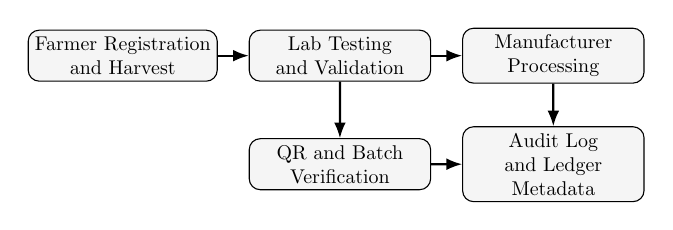
\begin{tikzpicture}[
scale=0.72,
transform shape,
node distance=0.7cm and 0.55cm,
box/.style={draw, rounded corners, align=center, minimum width=3.2cm, minimum height=0.9cm, fill=gray!8},
arrow/.style={-{Latex[length=2mm]}, thick}
]
\node[box] (farmer) {Farmer Registration\\and Harvest};
\node[box, right=of farmer] (lab) {Lab Testing\\and Validation};
\node[box, right=of lab] (manufacturer) {Manufacturer\\Processing};
\node[box, below=1.0cm of lab] (verify) {QR and Batch\\Verification};
\node[box, right=of verify] (audit) {Audit Log\\and Ledger\\Metadata};

\draw[arrow] (farmer) -- (lab);
\draw[arrow] (lab) -- (manufacturer);
\draw[arrow] (lab) -- (verify);
\draw[arrow] (manufacturer) -- (audit);
\draw[arrow] (verify) -- (audit);
\end{tikzpicture}
\caption{End-to-end workflow of the herb traceability platform.}
\label{fig:flowchart}
\end{figure}

\begin{figure}[!t]
\centering
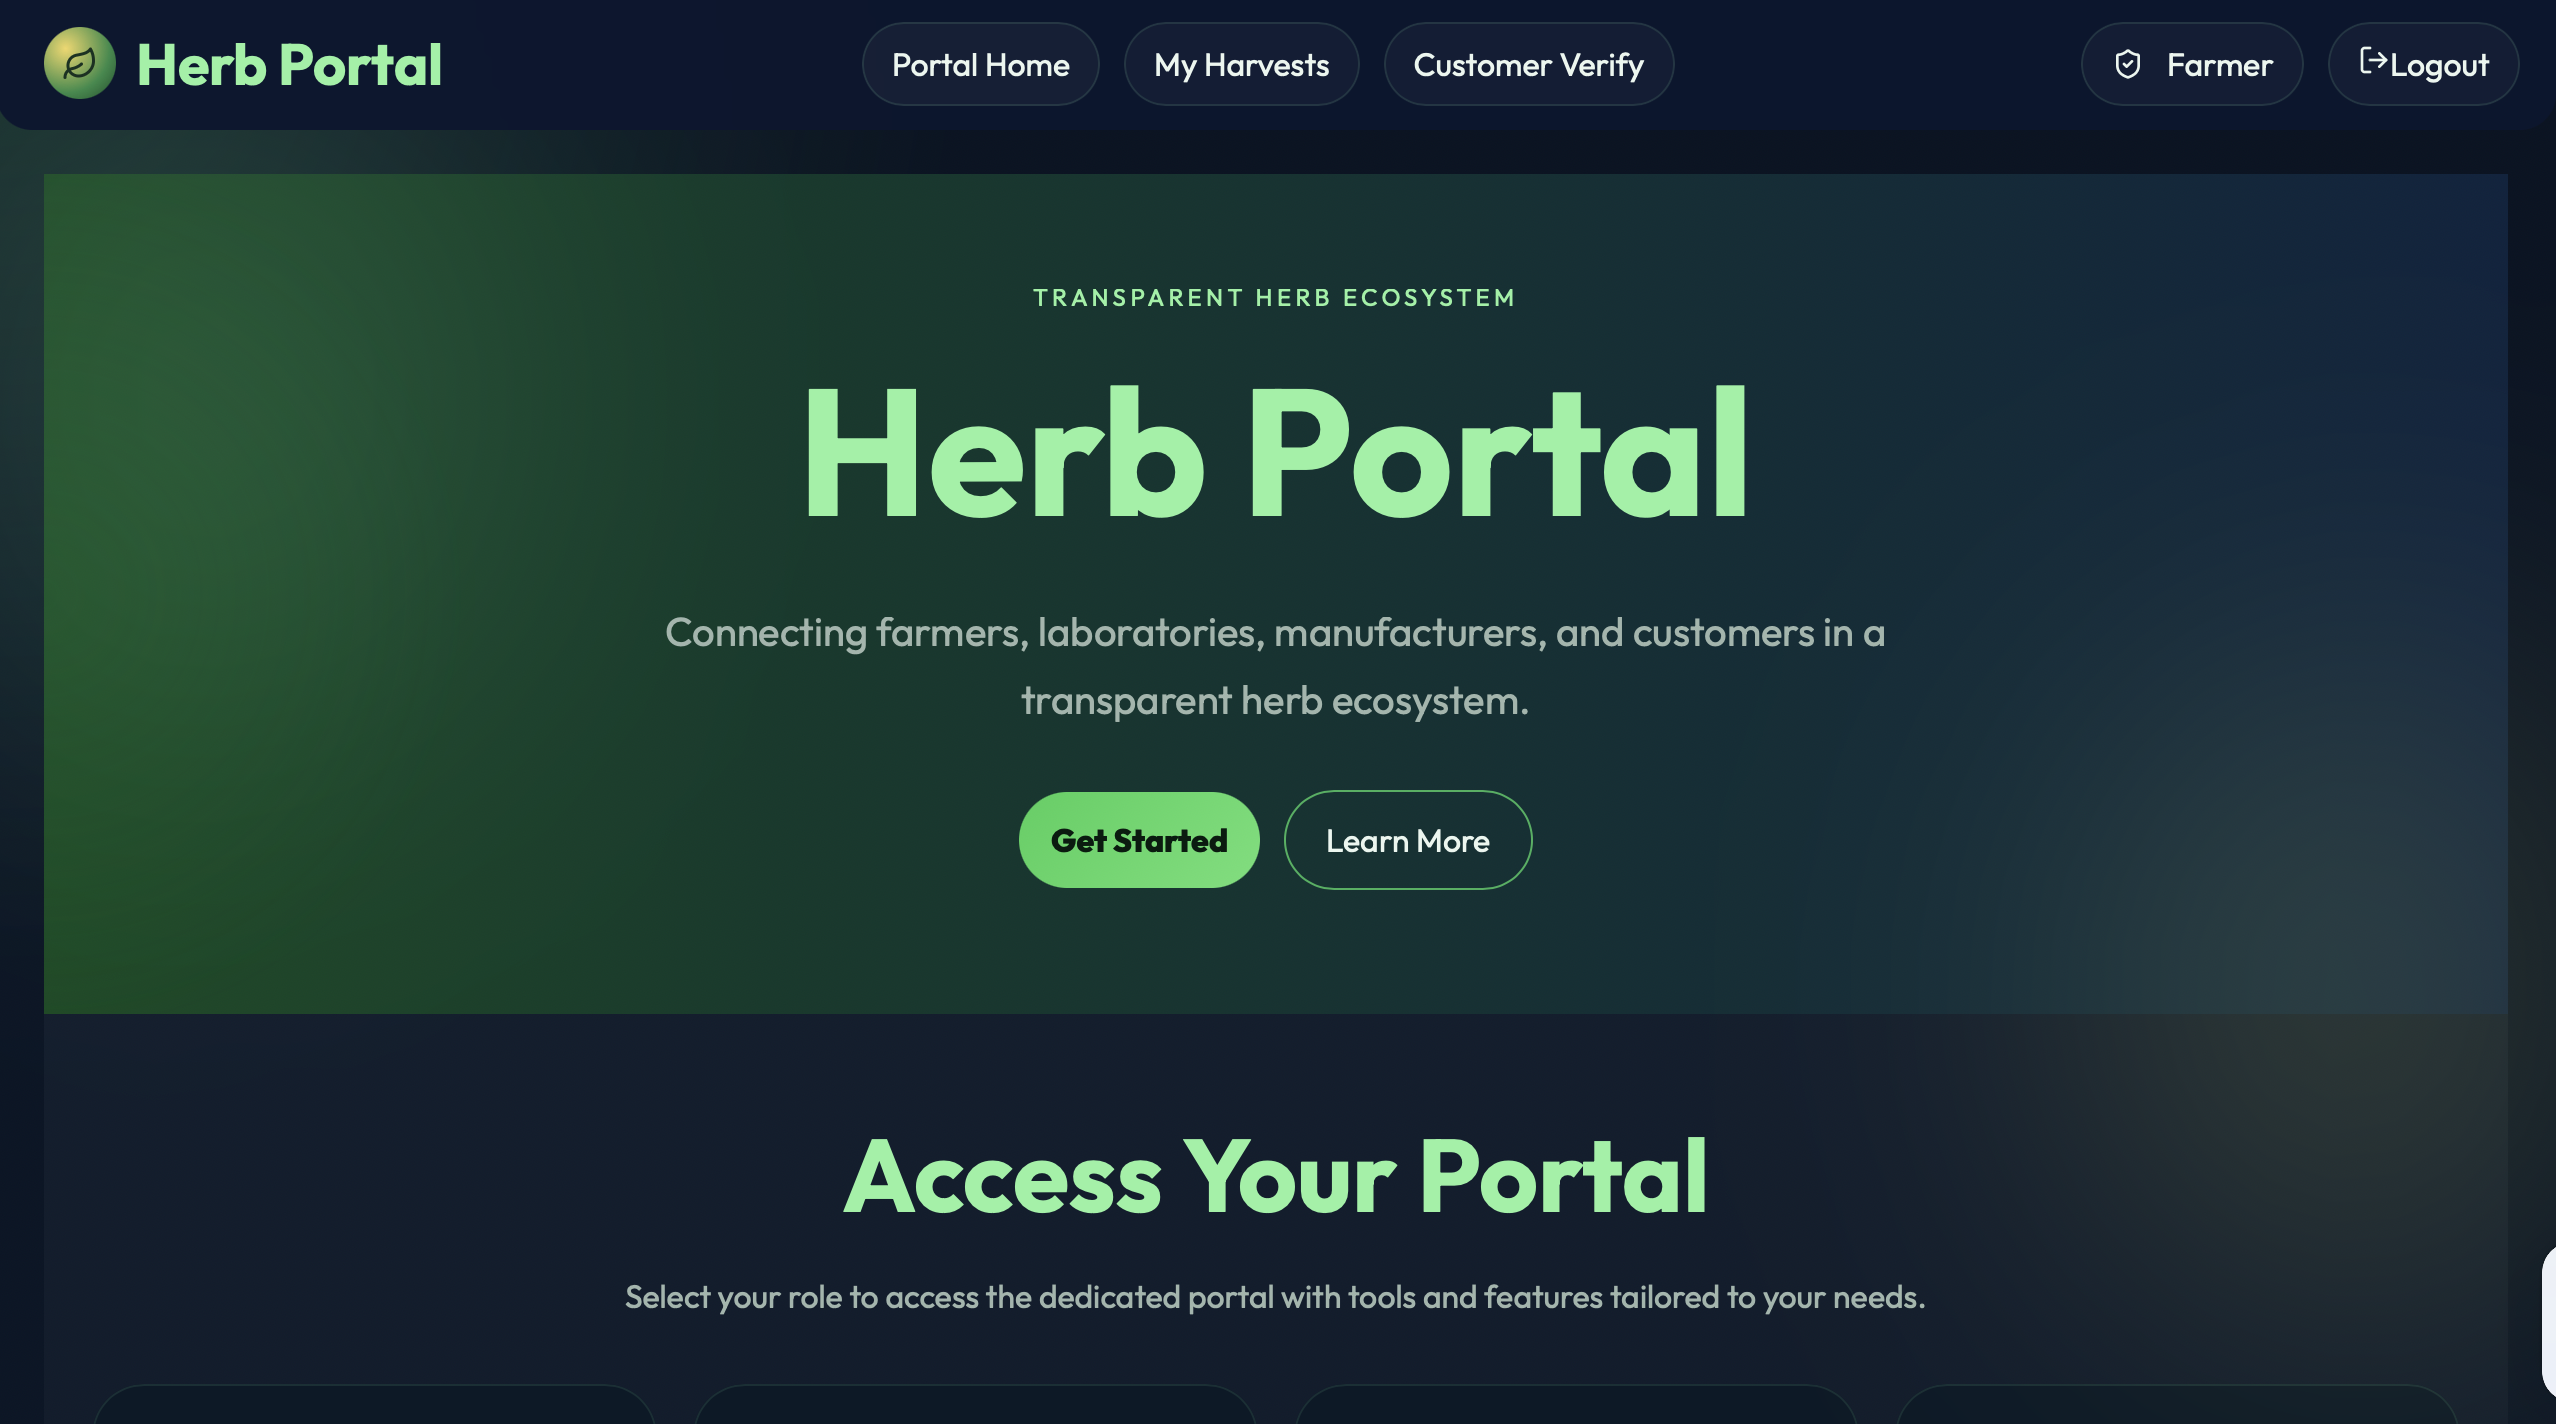
\includegraphics[width=\columnwidth]{docs/assets/home_page.png}
\caption{Landing page of the herb traceability platform.}
\label{fig:home}
\end{figure}

\begin{figure}[!t]
\centering
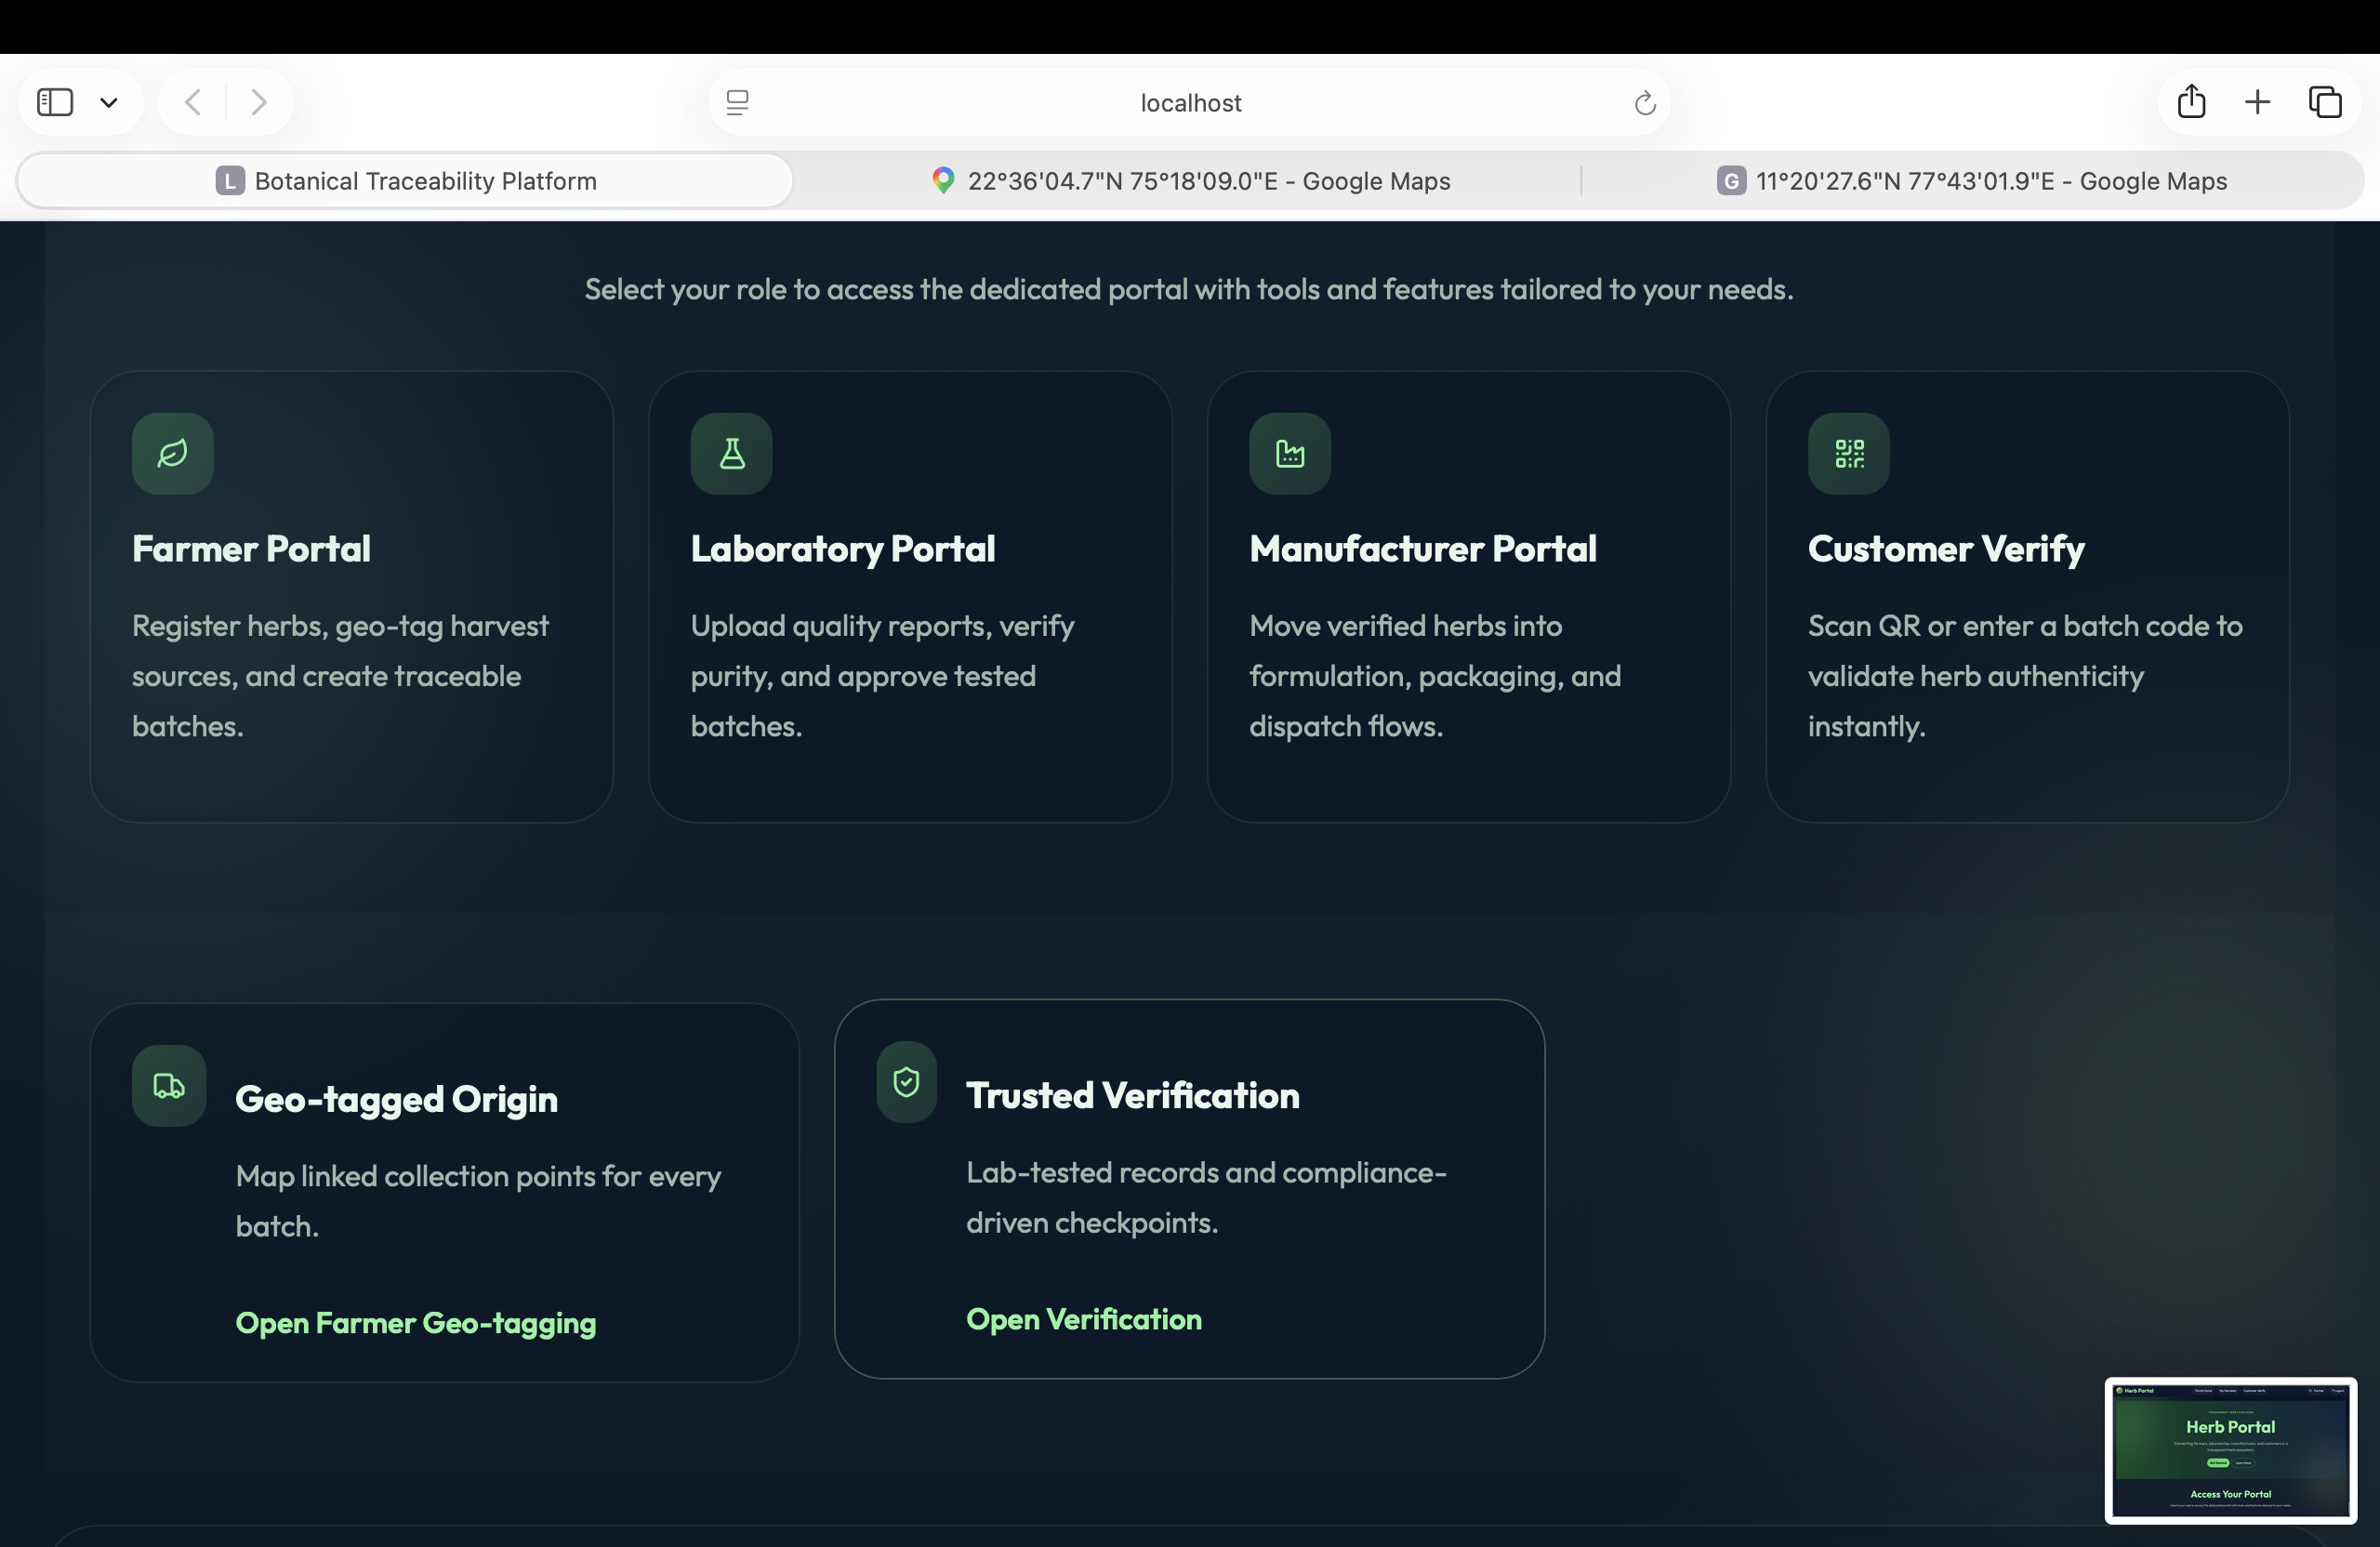
\includegraphics[width=\columnwidth]{docs/assets/portal_modules.png}
\caption{Role-based access modules for farmer, lab, manufacturer, and customer verification.}
\label{fig:portals}
\end{figure}

\begin{figure}[!t]
\centering
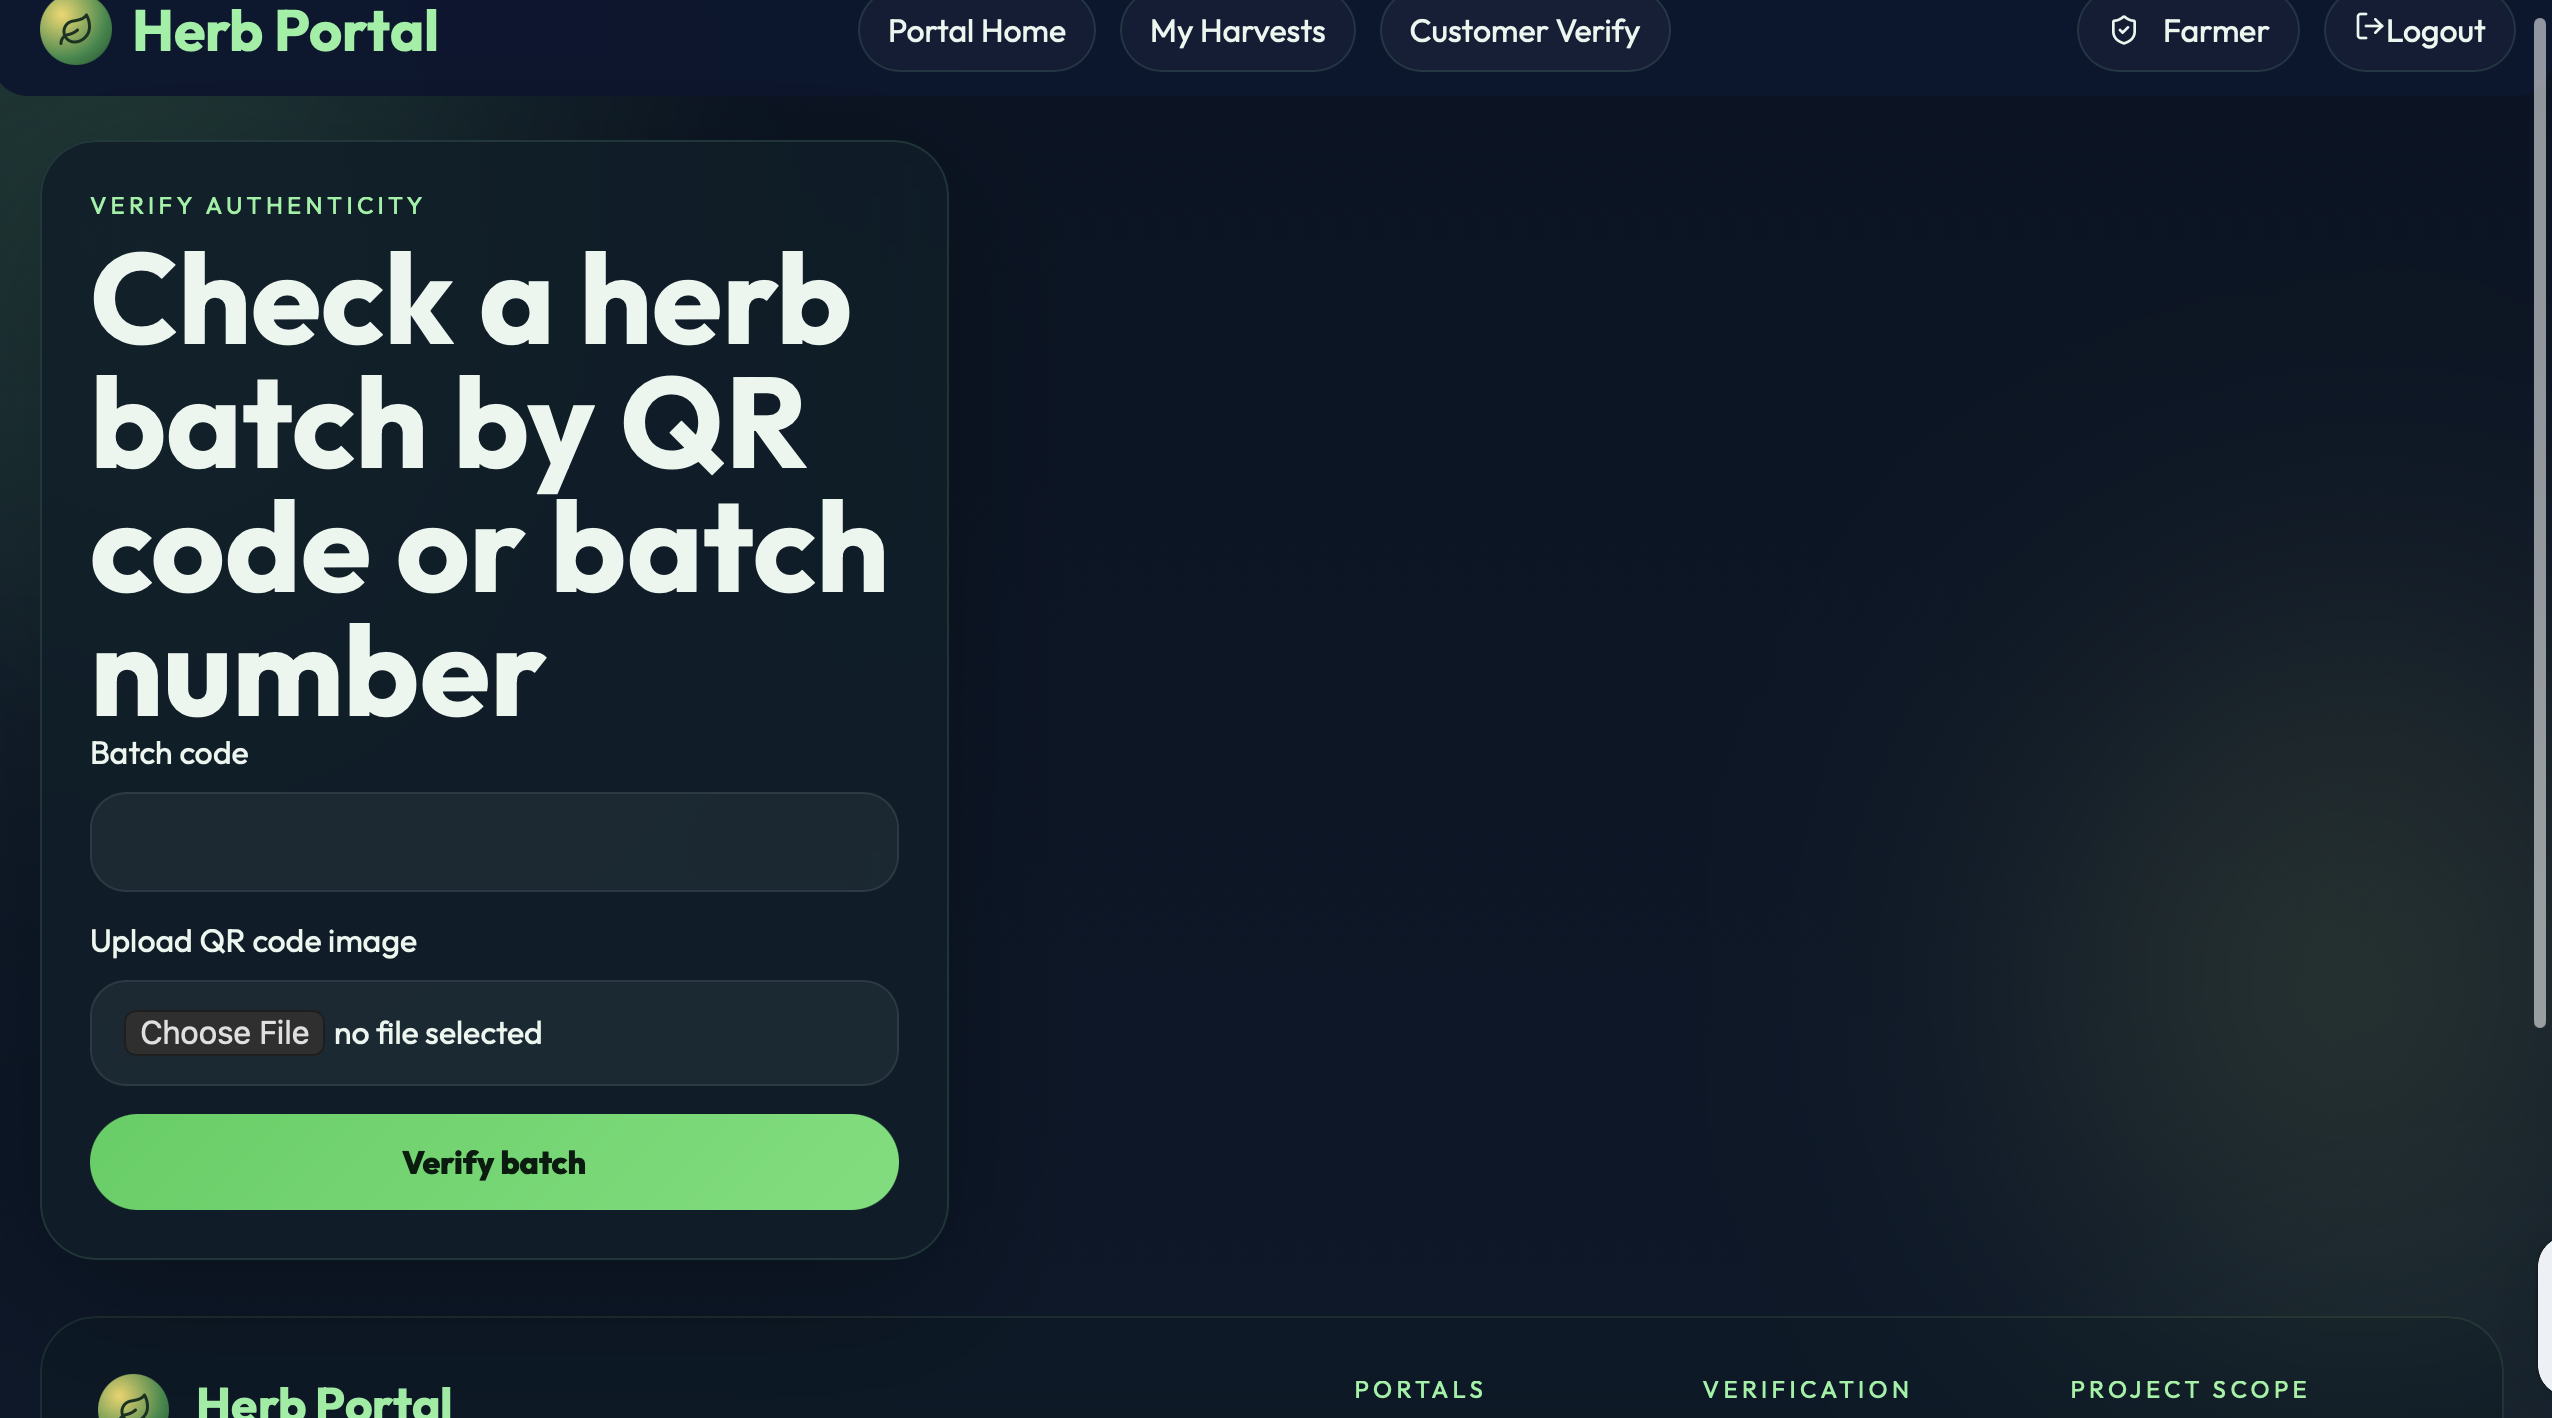
\includegraphics[width=\columnwidth]{docs/assets/customer_verify.png}
\caption{Customer verification screen for QR-based or manual batch lookup.}
\label{fig:verify}
\end{figure}

\begin{figure}[!t]
\centering
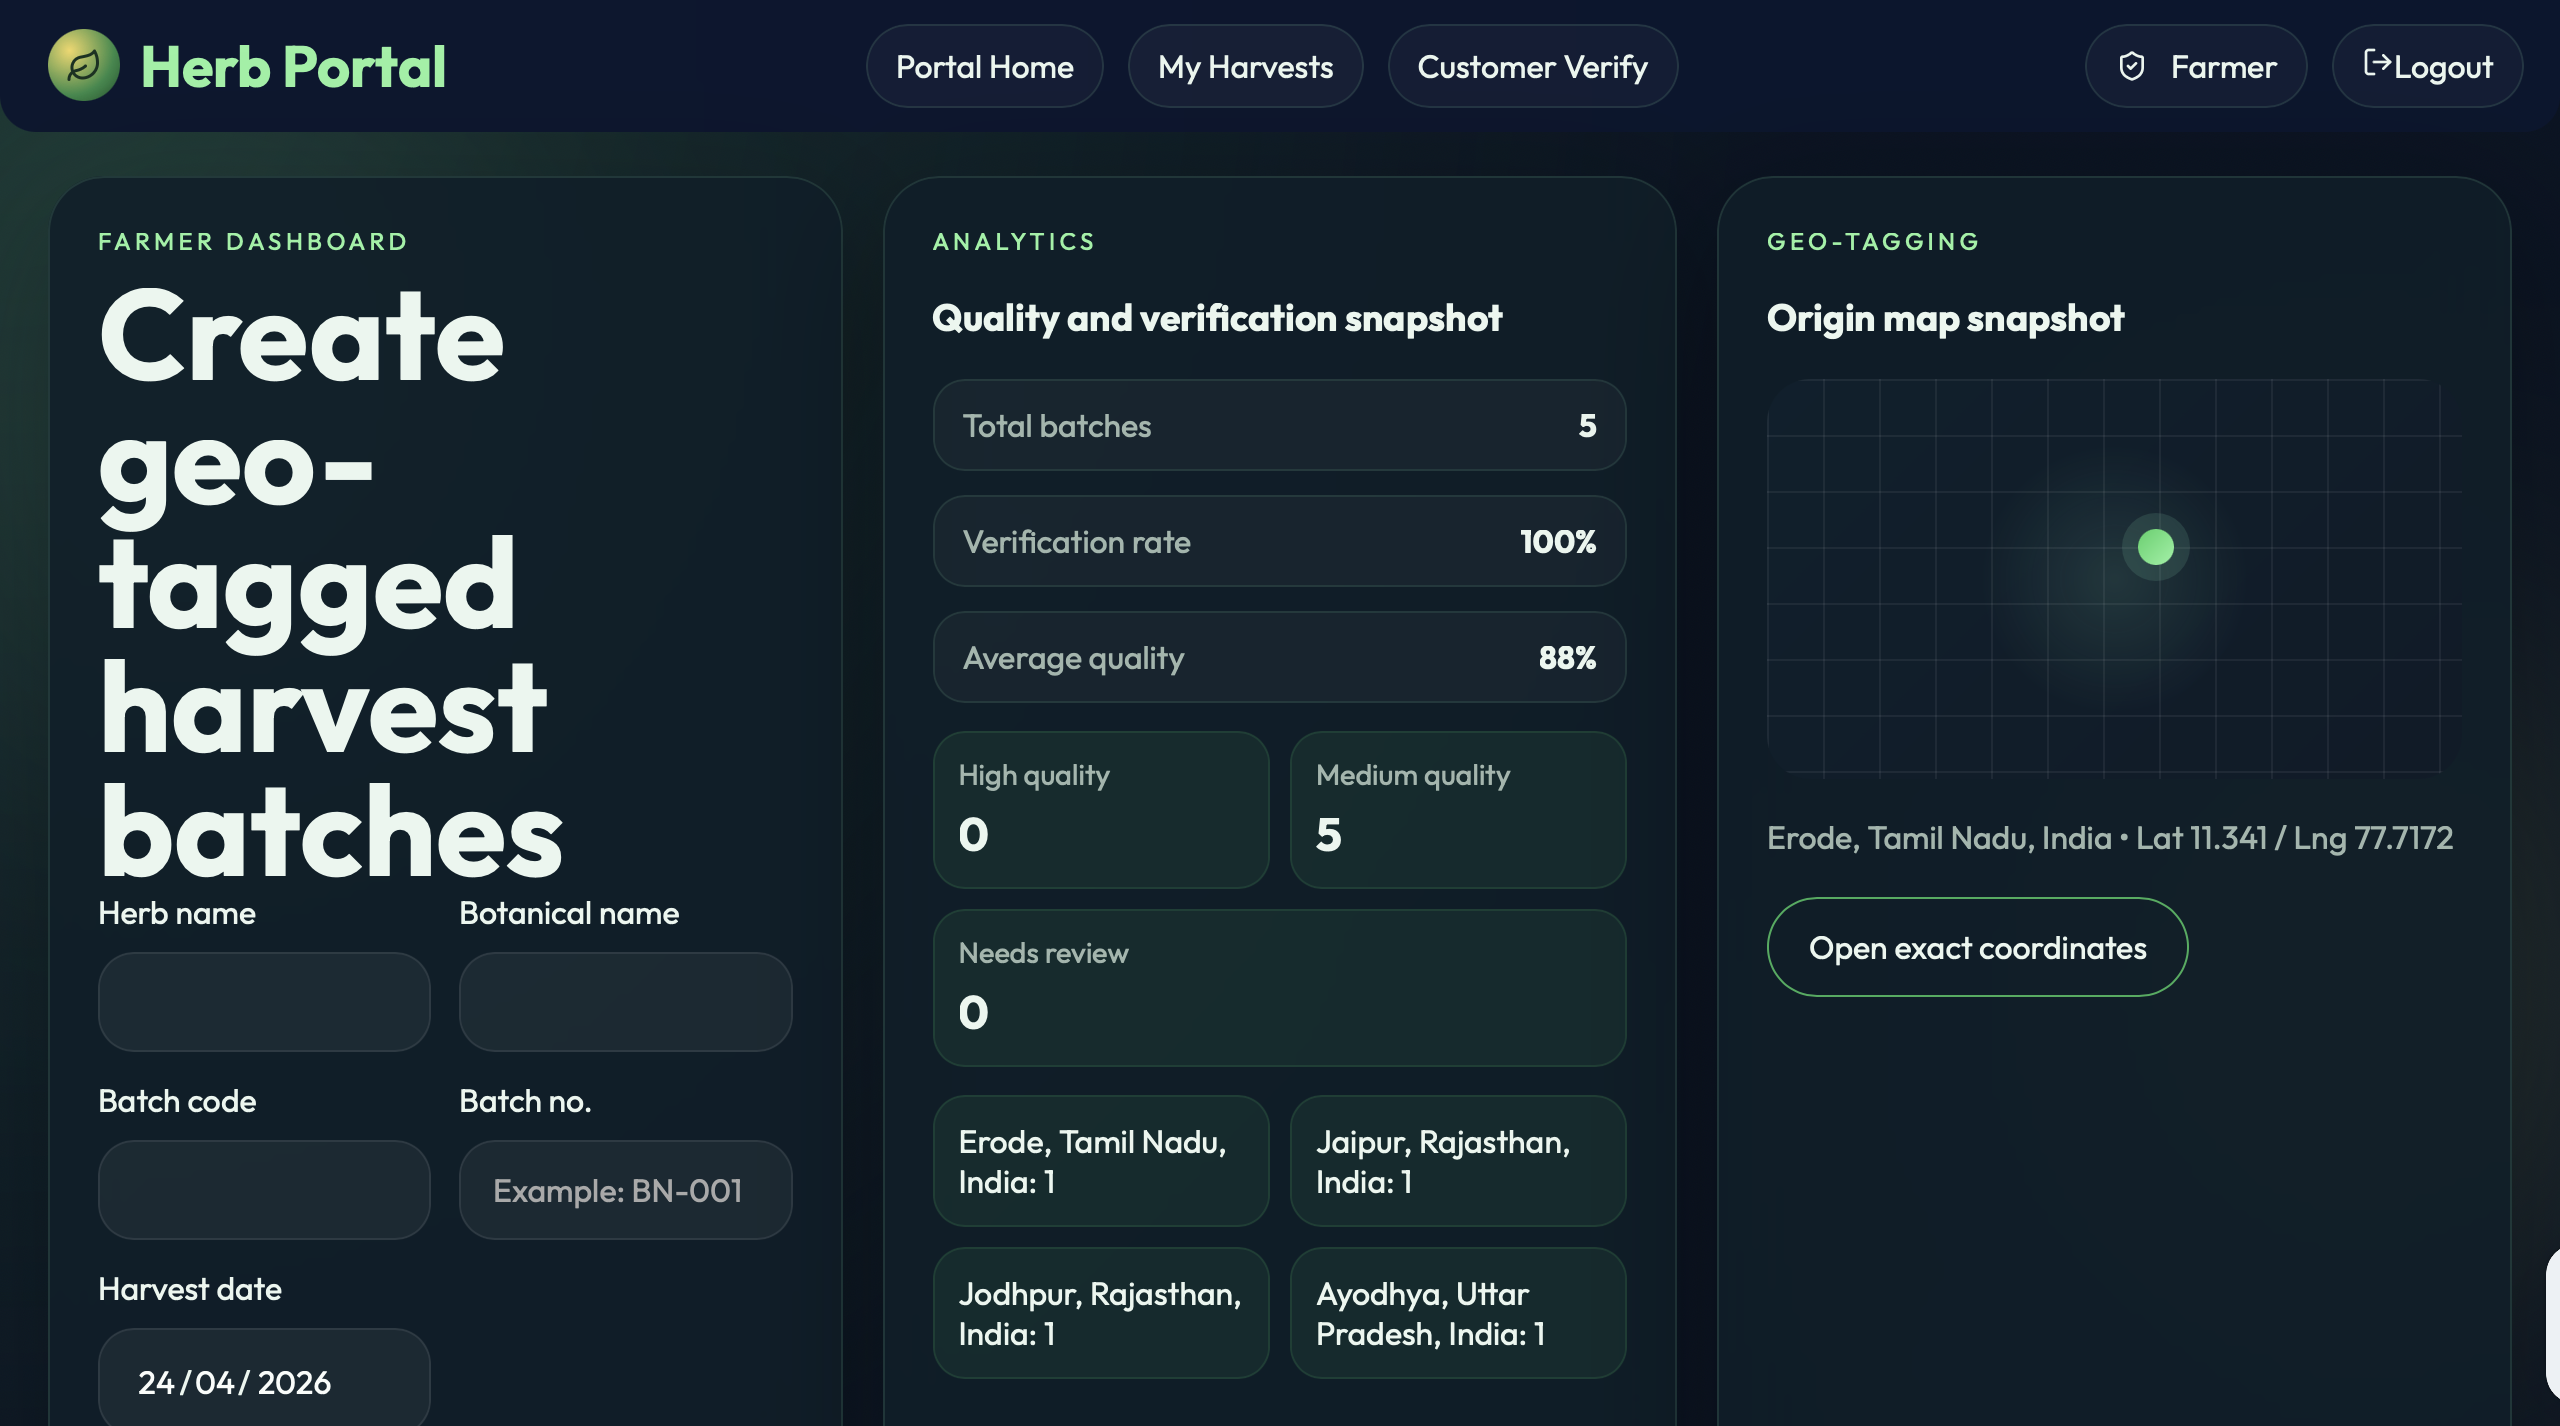
\includegraphics[width=\columnwidth]{docs/assets/farmer_dashboard.png}
\caption{Farmer dashboard with batch creation, analytics, and origin mapping.}
\label{fig:dashboard}
\end{figure}

\section{Conclusion}
This paper presented an IEEE-style research formulation of a herb traceability project designed for Ayurvedic and medicinal-plant supply chains. The work combines geo-tagged batch creation, laboratory reporting, manufacturer-side processing logs, customer verification, and blockchain-ready trace anchoring within a single batch-centered architecture. By structuring these functions around one persistent digital identity, the system addresses a central challenge repeatedly highlighted in recent literature: traceability fails when provenance, quality evidence, and downstream process records are separated across actors and tools.

The implemented prototype shows that a practical web platform can bridge that gap without excessive architectural complexity. React-based role dashboards make the workflow usable for different participants, while the Express and MongoDB backend preserves a continuous evidence trail through embedded reports, event logs, and audit entries. The QR verification interface then converts internal operational data into consumer-facing transparency, which is especially important in herbal markets where authenticity and safety directly affect trust. Although the present ledger integration is still preparatory, the availability of blockchain metadata and a smart-contract scaffold provides a realistic migration path toward tamper-evident anchoring.

Future work should focus on empirical deployment with real herbal cooperatives, direct blockchain execution, interoperability with regulatory datasets, and integration of sensor or vision-based quality intelligence. Large-sample usability studies, security evaluation, and performance benchmarking across mobile verification scenarios would also strengthen the evidence base for adoption. Even in its current form, the project demonstrates that digital traceability for herbs can be engineered as a coherent, auditable, and extensible system rather than a collection of disconnected records.

\begin{thebibliography}{00}
\bibitem{b1} P. Azevedo, J. Gomes, and M. Rom\~ao, ``Supply chain traceability using blockchain,'' \emph{Operations Management Research}, vol. 16, pp. 1359--1381, 2023, doi: 10.1007/s12063-023-00359-y.
\bibitem{b2} M. Vasileiou \emph{et al.}, ``Digital transformation of food supply chain management using blockchain: A systematic literature review towards food safety and traceability,'' \emph{Business \& Information Systems Engineering}, 2025, doi: 10.1007/s12599-025-00948-0.
\bibitem{b3} V. Sathiya \emph{et al.}, ``Tracking perishable foods in the supply chain using chain of things technology,'' \emph{Scientific Reports}, vol. 14, Art. no. 21621, 2024, doi: 10.1038/s41598-024-72617-3.
\bibitem{b4} L. Li \emph{et al.}, ``Design of agricultural product traceability system based on blockchain and RFID,'' \emph{Scientific Reports}, vol. 14, Art. no. 23599, 2024, doi: 10.1038/s41598-024-73711-2.
\bibitem{b5} A. Patel \emph{et al.}, ``Blockchain enabled traceability in the jewel supply chain,'' \emph{Scientific Reports}, vol. 15, Art. no. 3837, 2025, doi: 10.1038/s41598-025-88245-4.
\bibitem{b6} A. Rashid \emph{et al.}, ``Enhancing fruit supply chain traceability through blockchain and cryptographic protocols for achieving UN sustainable development goals,'' \emph{Scientific Reports}, vol. 16, Art. no. 7219, 2026, doi: 10.1038/s41598-026-37534-7.
\bibitem{b7} Z. El Hathat \emph{et al.}, ``Leveraging greenhouse gas emissions traceability in the groundnut supply chain: Blockchain-enabled off-chain machine learning as a driver of sustainability,'' \emph{Information Systems Frontiers}, vol. 26, pp. 2059--2076, 2024, doi: 10.1007/s10796-024-10514-w.
\bibitem{b8} M. Magdy, M. Grida, and G. Hussein, ``Disruption mitigation in the semiconductors supply chain by using public blockchains,'' \emph{The Journal of Supercomputing}, vol. 80, pp. 1852--1906, 2024, doi: 10.1007/s11227-023-05543-2.
\bibitem{b9} J. Chen \emph{et al.}, ``From capability to intention: A DCV-TAM hybrid model for blockchain adoption in circular agri-food supply chains,'' \emph{Agricultural and Food Economics}, vol. 14, Art. no. 34, 2026, doi: 10.1186/s40100-026-00471-0.
\bibitem{b10} M. S. Basir \emph{et al.}, ``From pen and paper to digital precision: A comprehensive review of on-farm recordkeeping,'' \emph{Precision Agriculture}, vol. 25, pp. 2643--2682, 2024, doi: 10.1007/s11119-024-10172-7.
\bibitem{b11} G. I. Edo \emph{et al.}, ``The use of quality control parameters in the evaluation of herbal drugs: A review,'' \emph{Discover Medicine}, vol. 1, Art. no. 168, 2024, doi: 10.1007/s44337-024-00177-6.
\bibitem{b12} C. Tan \emph{et al.}, ``Rapid identification of medicinal plants via visual feature-based deep learning,'' \emph{Plant Methods}, vol. 20, Art. no. 81, 2024, doi: 10.1186/s13007-024-01202-6.
\bibitem{b13} K. Komatsu, ``Comprehensive study on genetic and chemical diversity of Asian medicinal plants, aimed at sustainable use and standardization of traditional crude drugs,'' \emph{Journal of Natural Medicines}, vol. 78, pp. 267--284, 2024, doi: 10.1007/s11418-023-01770-2.
\bibitem{b14} H. Fuchino, ``Research on the quality evaluation of crude drugs,'' \emph{Journal of Natural Medicines}, vol. 79, pp. 15--27, 2025, doi: 10.1007/s11418-024-01845-8.
\bibitem{b15} D. Kirubakaran \emph{et al.}, ``Smart technologies enhance detection, monitoring, and traceability in global food safety,'' \emph{Discover Food}, vol. 6, Art. no. 41, 2026, doi: 10.1007/s44187-025-00716-9.
\end{thebibliography}

\end{document}
